 \documentclass{beamer}
\usepackage[latin1]{inputenc}
\usepackage{graphicx}
\usetheme{Warsaw}

\title{Sandpile Model}
\author{Yamin Zhou}\institute{University of Washington}

\begin{document}

\begin{frame}
\titlepage

\end{frame}

\begin{frame}
What is the sandpile model and why we care about sandpile model?
\end{frame}

\begin{frame}
The sandpile model,introduced in 1987,was the first model to exhibt self-organized critical behavior, that is, the system moved towards its critical point without the need to tune any adjustable external parameter.
\end{frame}


\begin{frame}
Let us use x,y to number the sites. Every cell can contain some chips, so the state of each cell has to be a non-negative interger Z(x,y) Starting with a flat surface Z(x,y)=0 for all x and y,in every time step a cell is randomly chosen and is incremented as shown in formula$$z\left ( x,y \right )\rightarrow z\left ( x,y \right )+1$$
Any site with$$z\left ( x,y \right )\geq 4$$ is unstable and can topple, sending one of its chips to each of its 4 neighbors:
$$z\left ( x,y \right )\rightarrow z\left ( x,y \right )-4$$
$$z\left ( x\pm 1,y \right )\rightarrow z\left ( x\pm 1,y \right )+1$$
$$z\left ( x,y \pm 1\right )\rightarrow z\left ( x,y\pm 1 \right )+1$$
\end{frame}


\begin{frame}
What is interesting about this model is which grain of sand will cause any one area to become unstable is unknown. This is due to the randomness of the location of each additional grain of sand. Although it is known with certainty eventually one grain of sand will cause collapse somewhere on the sandpile, where and when collapse will occur is unpredictable. Additionally, once one area becomes unstable the entire system is at risk of becoming unstable as well. This is because each area is connected and dependent on each other for stability.
\end{frame}

\begin{frame}
\begin{center}
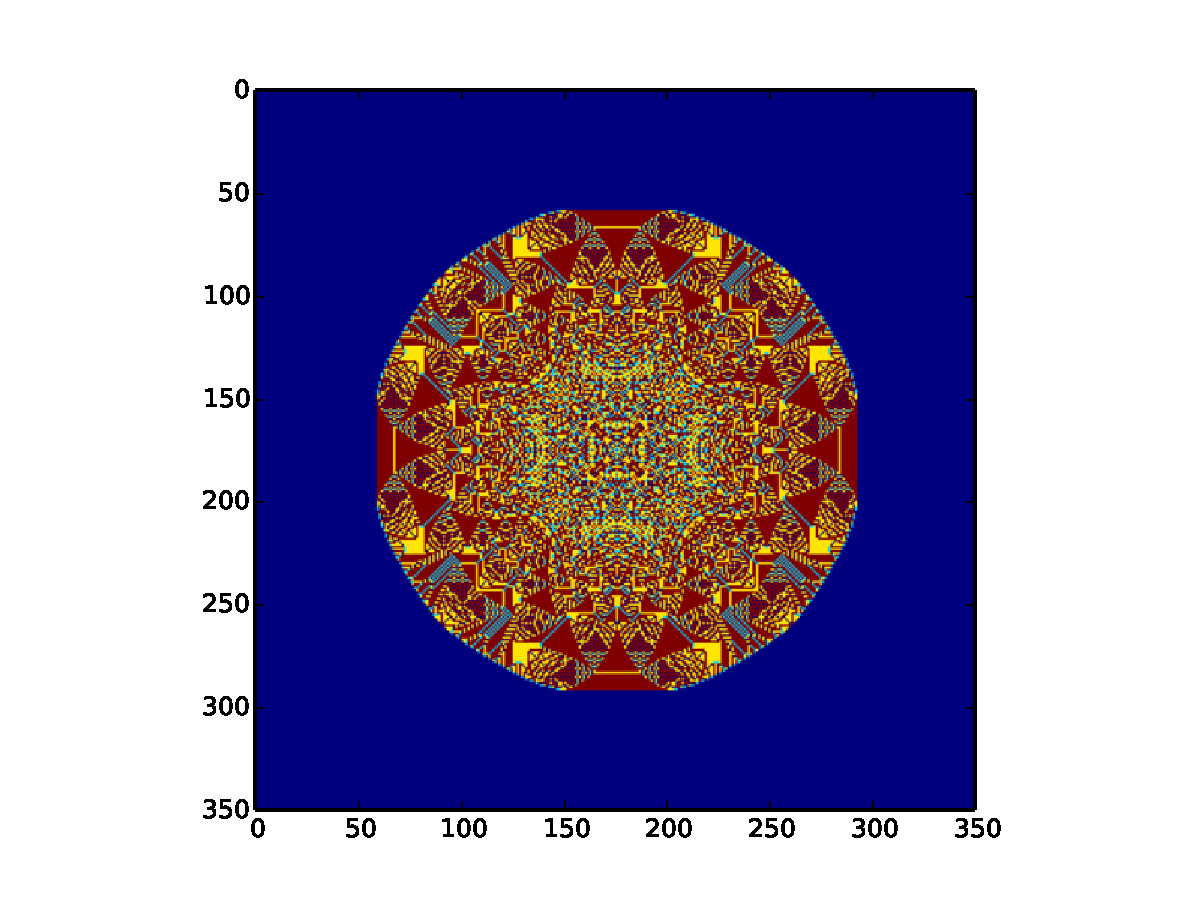
\includegraphics[scale = 0.5]{pic_sandpile}
\end{center}
\end{frame}

\begin{frame}
\begin{center}
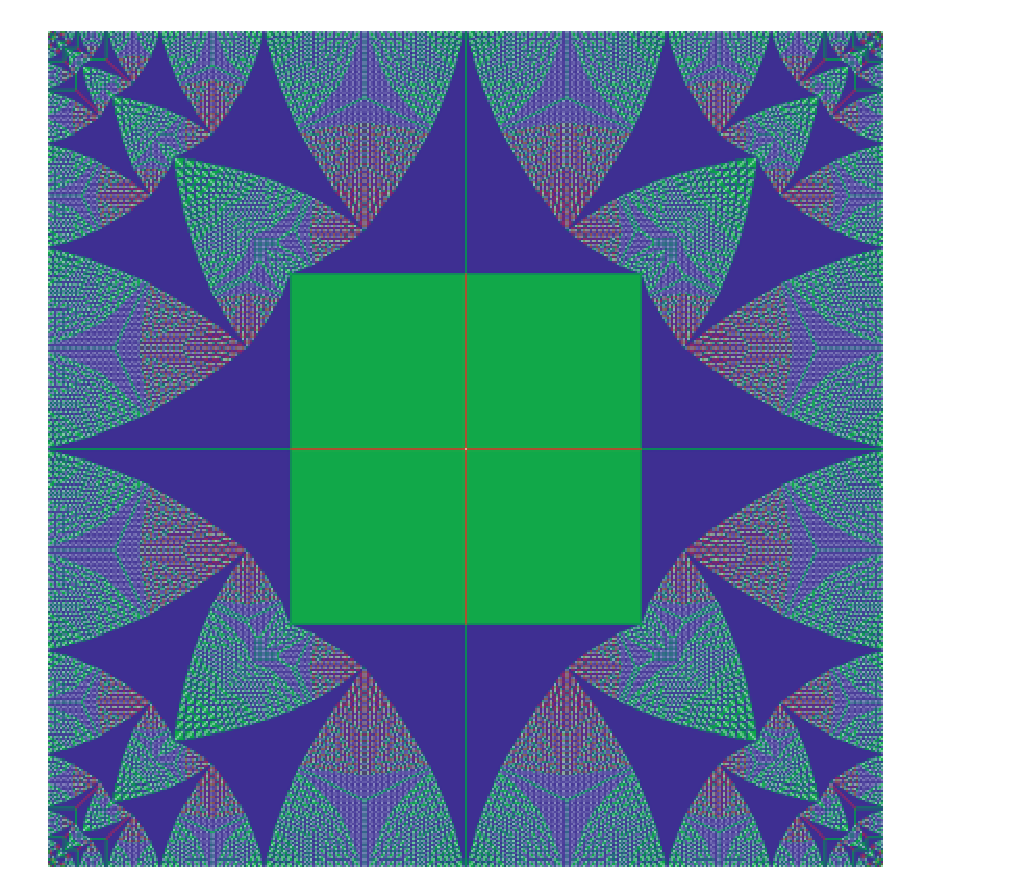
\includegraphics[scale = 0.5]{sandpile2}
\end{center}
\end{frame}

\begin{frame}
This is a very simple model that describe real phonenomenons incredibly well. Lots of natural events follow a power-law and so does the sandpile model.
\end{frame}

\begin{frame}
The Gutenberg-Richter law is $$log_{10} N(m)=a-b*m$$ where N(m)is the number of earthquakes per unit time interval with a magnitude greater than or equal to m,and a and b are parameters. 
\end{frame}

\begin{frame}
\begin{center}
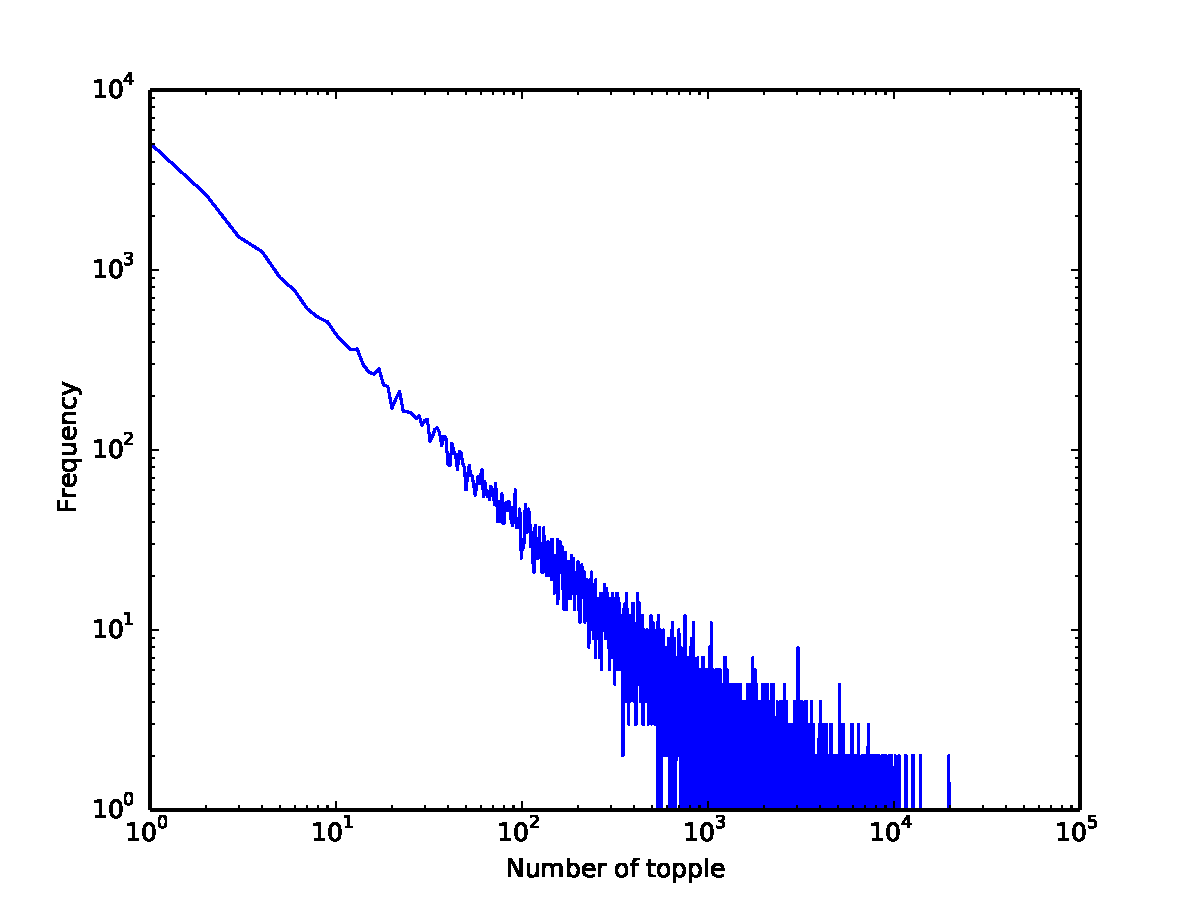
\includegraphics[scale = 0.5]{freq}
\end{center}
\end{frame}

\begin{frame}
This model has some characteristics.One of the remarketable results is, that after a while the average number of grains per site is almost stable.
\end{frame}

\begin{frame}
\begin{center}
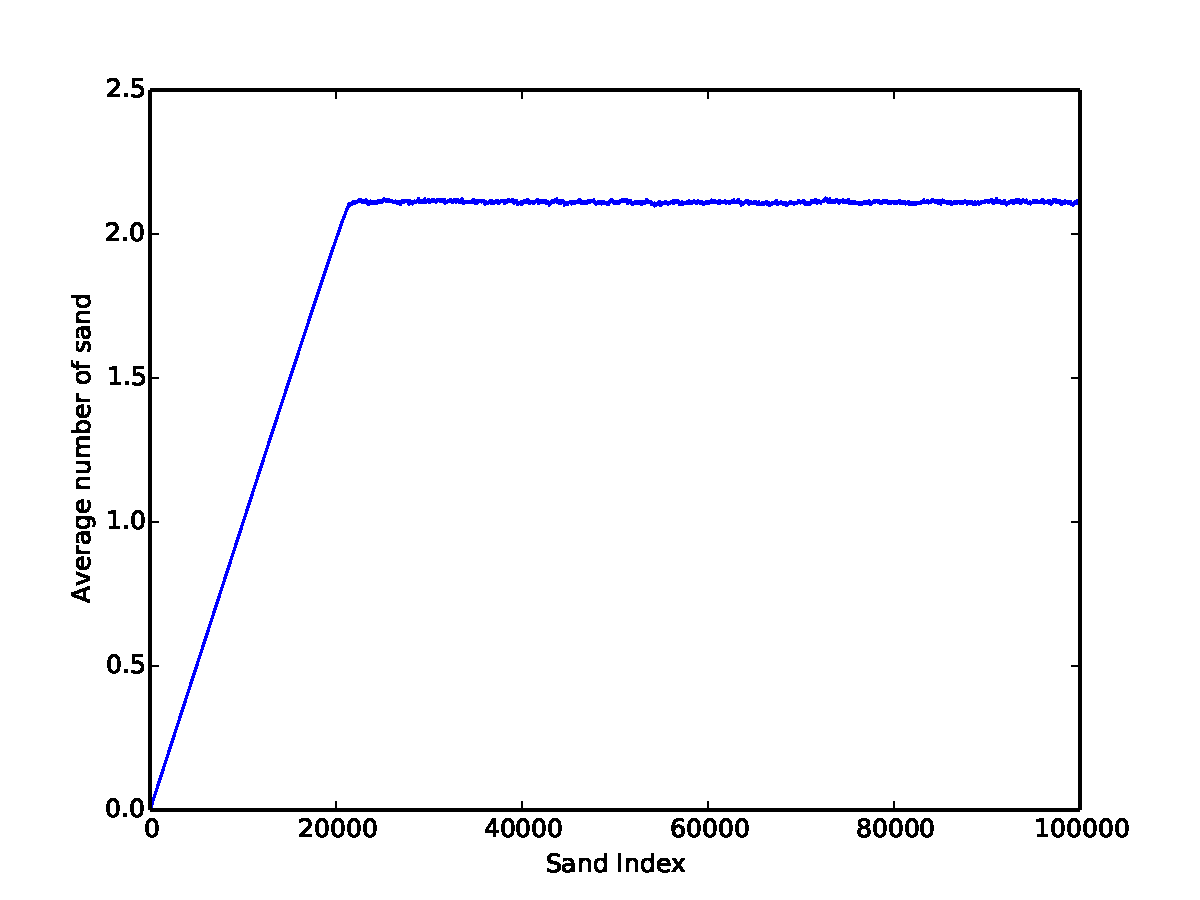
\includegraphics[scale = 0.5]{avg}
\end{center}
\end{frame}

\begin{frame}
References:\\
$http://en.wikipedia.org/wiki/Abelian_sandpile_model$
$http://www.ams.org/notices/201008/rtx100800976p.pdf$
\end{frame}

\end{document}
%sagemathcloud={"zoom_width":95}